%!TEX root=paper.tex

    \begin{figure*}[ht!]
      \centering
      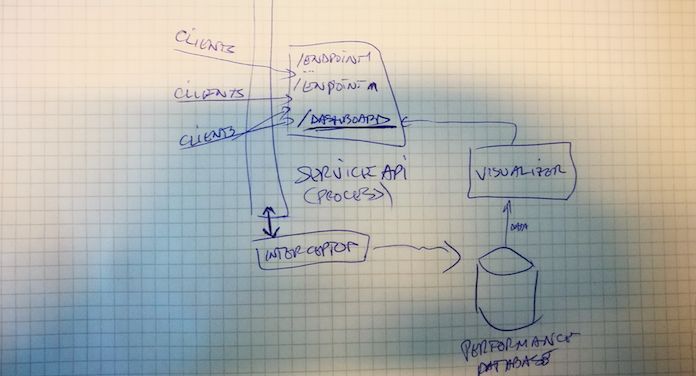
\includegraphics[width=0.8\linewidth]{interceptor}
      \caption{The first thing that needs to be done, is to decorate the application object with an INTERCEPTOR}
      \label{fig:sep}
    \end{figure*}


\section{Architecture}

REMEMBER THE GOAL: Our main goal with the \tool issues to allow the integration of the dashboard with an API with minimal effort.

The fact that the \tool itself is being developed in Python using Flask makes binding to the services of a to-be monitored application developed with the same technologies easy and intuitive. However, by writing different backends that do the measurement and monitoring, the frontend can be reused. 

The viewpoints we showed are only a subset of all the viewpoints of the \tool. In practice, the tool provides other perspectives as long as they are a combination of: 

\begin{itemize}
  \item Cardinality: one endpoint vs multiple
  \item Objective: utilization vs. performance (response time)
  \item Evolution Axis: time vs. versions
  \item Grouping: Grouped (e.g. by user) vs. All
\end{itemize}






\ins{The first important question that such a 
service monitoring system should provide is 
information about what endpoints are being
used and by whom}. 

TODO: Find references, arguments, related work
that provide more details about why understanding
who uses endpoints, and which are used are important.

This is clearly the case in static analysis (see paper
by haenni and lungu...) but should even more be the
case in APIs.




  \newpage


  % This used to be in the first section... 
  % Maybe it fits better localized here: 
  Data collected by the wrappers are persisted in a local database. The SQLAlchemy Object Relational Mapper\footnote{\url{https://www.sqlalchemy.org/}} allows for a DB system independent solution. 

  By default the system is deployed with an SQLite database \footnote{\url{https://www.sqlite.org/}} is used for this purpose.

TODO: TALK ABOUT THE METAMODEL...


    \begin{figure}[ht!]
      \centering
        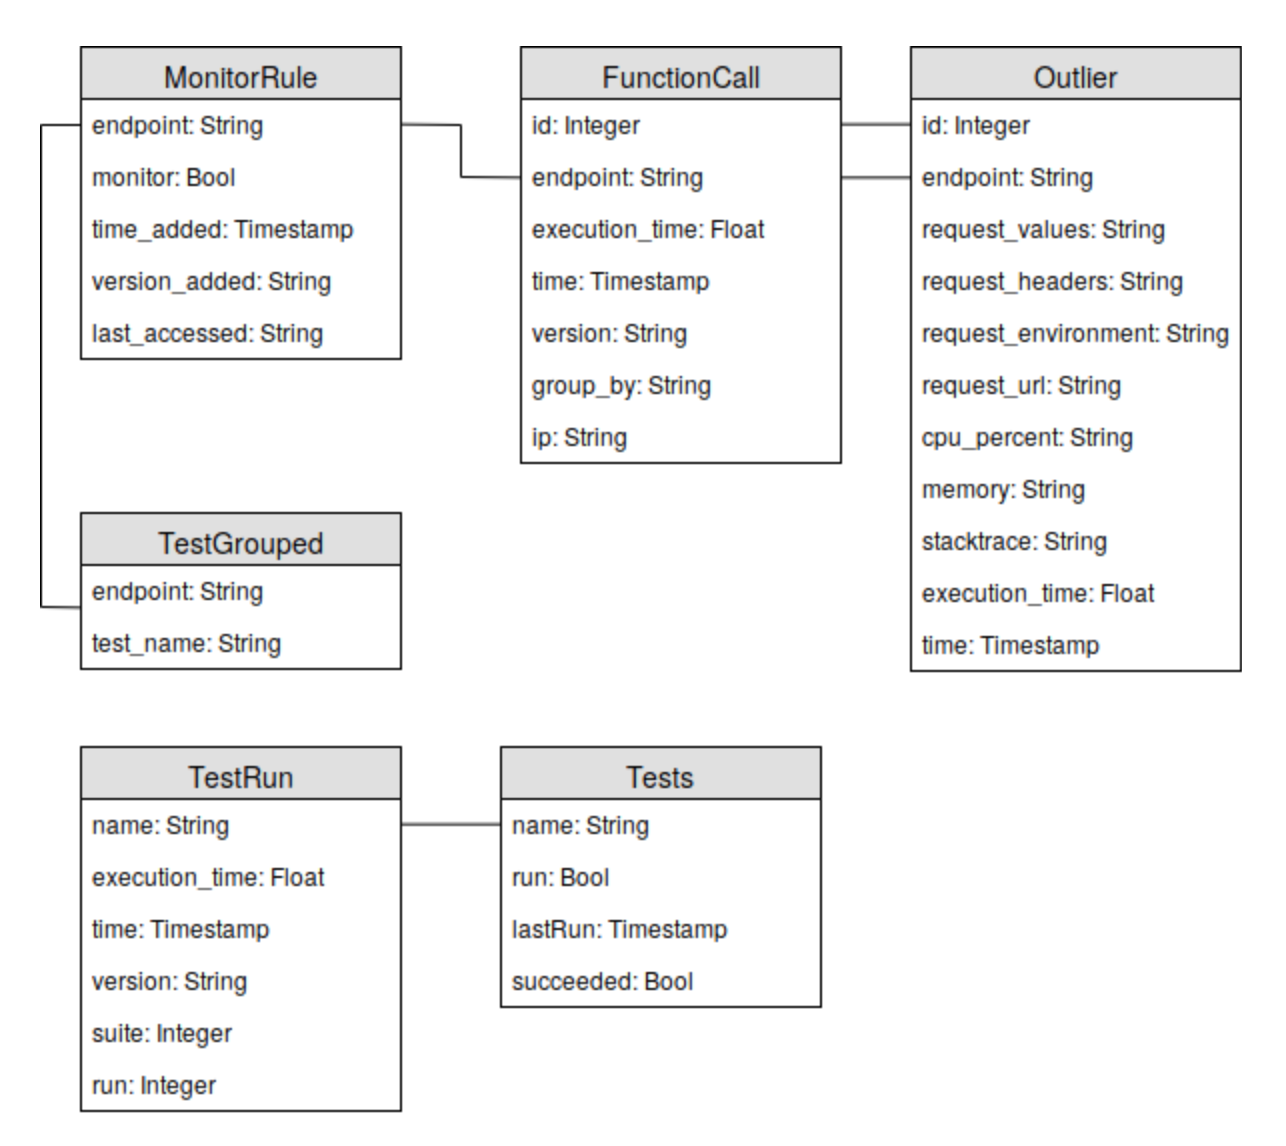
\includegraphics[width=0.8\linewidth]{db_schema}
        \caption{The model that supports the views presented in this paper}
        \label{fig:sep}
    \end{figure}

  As discussed in the introductory section, in previous work \withheld we introduced \tool, a drop-in Python library that allows developers to monitor their Flask-based Python web applications with minimal effort.
%
  The \tool is implemented for Python 3.6 and is available on the Python Package Index repository
  % \footnote{\url{https://pypi.python.org/pypi/flask-monitoring-dashboard/1.8}} 
  \footnote{\url{https://pypi.python.org/pypi/[\witheld]}} 
  from where it can be installed by running \install from the command line. 
%  
  The source code of the \tool is published under a permissive MIT license and is available on GitHub\footnote{\url{https://github.com/flask-dashboard}}.
  
  


